\documentclass[border=3mm]{standalone}
\usepackage{tikz}
\usetikzlibrary{arrows, shapes.gates.logic.US, shapes.gates.logic.IEC, calc}

\tikzset{
    my-nand-gate/.style={
        nand gate US, draw, rotate=0, logic gate inputs=nn
    },
    my-branch/.style={
        fill, shape=circle, minimum size=3pt, inner sep=0pt
    },
}

\begin{document}

\resizebox{16cm}{!}{

    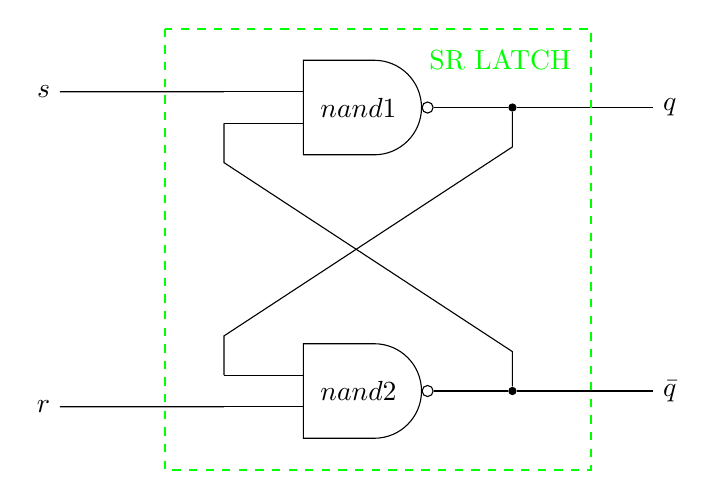
\begin{tikzpicture}[label distance=2mm]

        % INPUTS
        \node[] (S) at (0, 0)            {\normalsize $s$};
        \node[] (R) at ($(S) + (0, -4)$) {\normalsize $r$};

        % NAND1, WIRES AND CONNECTOR POINTS
        \node[my-nand-gate] (NAND1)    at ($(S) + (4, -.2)$)            {\normalsize $nand1$};
        \coordinate[]       (NAND1IN1) at ($(NAND1.input 1) + (-1, 0)$) {};
        \coordinate[]       (NAND1IN2) at ($(NAND1.input 2) + (-1, 0)$) {};
        \node[my-branch]    (NAND1OUT) at ($(NAND1.output)  + (1, 0)$)  {};
        \draw (NAND1.input 1) -- (NAND1IN1);
        \draw (NAND1.input 2) -- (NAND1IN2);
        \draw (NAND1.output)  -- (NAND1OUT);
        
        % NAND2, WIRES AND CONNECTOR POINTS
        \node[my-nand-gate] (NAND2)    at ($(R) + (4, .2)$)             {\normalsize $nand2$};
        \coordinate[]       (NAND2IN1) at ($(NAND2.input 1) + (-1, 0)$) {};
        \coordinate[]       (NAND2IN2) at ($(NAND2.input 2) + (-1, 0)$) {};
        \node[my-branch]    (NAND2OUT) at ($(NAND2.output)  + (1, 0)$)  {};
        \draw (NAND2.input 1) -- (NAND2IN1);
        \draw (NAND2.input 2) -- (NAND2IN2);
        \draw (NAND2.output)  -- (NAND2OUT);

        % OUTPUTS
        \node[] (Q)    at ($(NAND1OUT) + (2, 0)$) {\normalsize $q$};
        \node[] (QBAR) at ($(NAND2OUT) + (2, 0)$) {\normalsize $\bar{q}$};
                
        % INPUT CONNECTIONS
        \draw (S) -- (NAND1IN1);
        \draw (R) -- (NAND2IN2);
        
        % OUTPUT CONNECTIONS
        \draw (NAND1OUT) -- (Q);
        \draw (NAND2OUT) -- (QBAR);

        % INTERNAL WIRES - NAND GATE
        \draw (NAND1OUT) -- ++(0,-0.5) -- ($(NAND2IN1) +(0,0.5)$)  -- (NAND2IN1);
        \draw (NAND2OUT) -- ++(0,0.5)  -- ($(NAND1IN2) +(0,-0.5)$) -- (NAND1IN2);

        % DRAW DOTTED LINE BOX AROUND SR LATCH
        \draw[thick, dashed, green] ($(NAND1IN1) + (-.75, .8)$) rectangle ($(NAND2OUT) + (1, -1)$);
        \node[green] at ($(NAND1) + (1.8, .6)$) {\normalsize SR LATCH};

    \end{tikzpicture}
}

\end{document} 
